%% ----------------------------------------------------------------
%% Thesis.tex -- MAIN FILE (the one that you compile with LaTeX)
%% ----------------------------------------------------------------

% Set up the document
% Use the "Thesis" style, based on the ECS Thesis style by Steve Gunn
\documentclass[a4paper, 11pt, oneside]{Thesis}
% Location of the graphics files (set up for graphics to be in PDF format)
\graphicspath{{Figures/}}

% Include any extra LaTeX packages required
% Use the "Natbib" style for the references in the Bibliography
\usepackage[square, numbers, comma, sort&compress]{natbib}
% Needed for the "comment" environment to make LaTeX comments
\usepackage{verbatim}
% Allows "\bvec{}" and "\buvec{}" for "blackboard" style bold vectors in maths
\usepackage{vector}
% Colours hyperlinks in blue, but this can be distracting if there are many
% links.
\hypersetup{urlcolor=blue, colorlinks=true}

%% ----------------------------------------------------------------
\begin{document}
% Begin Roman style (i, ii, iii, iv...) page numbering
\frontmatter

% Set up the Title Page
\title  {Skill Social Network} \authors  {\texorpdfstring
{\href{dima@ceata.org}{Dumitru Ursu}} {Dumitru Ursu} }
% Do not change this here, instead these must be set in the "Thesis.cls" file,
% please look through it instead
\addresses  {\groupname\\\deptname\\\univname} \date       {\today} \subject
{} \keywords   {}

\maketitle
%% ----------------------------------------------------------------
% It is better to have smaller font and larger line spacing than the other way
% round
\setstretch{1.3}

% Define the page headers using the FancyHdr package and set up for one-sided
% printing
\fancyhead{}  % Clears all page headers and footers \rhead{\thepage}  % Sets the
right side header to show the page number \lhead{}  % Clears the left side page
header

 % Finally, use the "fancy" page style to implement the FancyHdr headers
\pagestyle{fancy}

%% ----------------------------------------------------------------
% Declaration Page required for the Thesis, your institution may give you a
% different text to place here
\Declaration{

\addtocontents{toc}{\vspace{1em}}  % Add a gap in the Contents, for aesthetics

I, Dumitru Ursu, declare that this thesis titled, `Skill social network' and the
work presented in it are my own. I confirm that:

\begin{itemize}
\item[\tiny{$\blacksquare$}] This work was done wholly or mainly
            while in candidature for a research degree at this University.

\item[\tiny{$\blacksquare$}] Where any part of this thesis has previously been
    submitted for a degree or any other qualification at this University or any
    other institution, this has been clearly stated.

\item[\tiny{$\blacksquare$}] Where I have consulted the published work of
    others, this is always clearly attributed.

\item[\tiny{$\blacksquare$}] Where I have quoted from the work of others, the
    source is always given. With the exception of such quotations, this thesis
    is entirely my own work.

\item[\tiny{$\blacksquare$}] I have acknowledged all main sources of help.

\item[\tiny{$\blacksquare$}] Where the thesis is based on work done by myself
jointly with others, I have made clear exactly what was done by others and what
I have contributed myself.  \\
\end{itemize}

Signed:\\ \rule[1em]{25em}{0.5pt}  % This prints a line for the signature

Date:\\ \rule[1em]{25em}{0.5pt}  % This prints a line to write the date
}
\clearpage  % Declaration ended, now start a new page

%% ----------------------------------------------------------------
% The "Funny Quote Page"
\pagestyle{empty}  % No headers or footers for the following pages

\null\vfill
% Now comes the "Funny Quote", written in italics
\textit{``Aut disce aut discede''}\\
\textit{``Either learn or go away''}


\begin{flushright} Latin saying \end{flushright}

\vfill\vfill\vfill\vfill\vfill\vfill\null
\clearpage  % Funny Quote page ended,
%% ----------------------------------------------------------------

% The Abstract Page
\addtotoc{Abstract} % Add the "Abstract" page entry to the Contents
\abstract{
\addtocontents{toc}{\vspace{1em}} % Add a gap in the Contents, for aesthetics

This thesis covers the design and implementation of a peer-to-peer teaching
network. The primary goals is to use cutting-edge technology in order to create
the social network and to explore unconventional virtual learning techniques.
One of the secondary goals of the system is to make it standard-based, web-only,
and so to make it accessible, and independent of proprietary technology.

In order to make the software more useful, it is released under a Free Software
license, \href{http://www.gnu.org/licenses/agpl-3.0.html}{AGPLv3}. The code can
be downloaded from \href{https://gitorious.org/discite/discite/}{Gitorious}, and
used without restrictions by universities or high schools. Deployment scripts
are provided, and so is documentation.

An instance of the application is running at \url{http://discite.info}. The
name of the application, "Discite", means "to learn" in Latin.

}

\clearpage  % Abstract ended, start a new page
%% ----------------------------------------------------------------

% Reset the line-spacing to 1.3 for body text (if it has changed)
\setstretch{1.3}

% The Acknowledgements page, for thanking everyone
\acknowledgements{
\addtocontents{toc}{\vspace{1em}}  % Add a gap in the Contents, for aesthetics

The acknowledgements and the people to thank go here, don't forget to include
your project advisor\ldots

}
\clearpage  % End of the Acknowledgements
%% ----------------------------------------------------------------

% The page style headers have been "empty" all this time, now use the "fancy"
% headers as defined before to bring them back
\pagestyle{fancy}


%% ----------------------------------------------------------------
\lhead{\emph{Contents}}  % Set the left side page header to "Contents"
\tableofcontents  % Write out the Table of Contents

%% ----------------------------------------------------------------
% Set the left side page header to "List if Figures"
\lhead{\emph{List of Figures}}
\listoffigures  % Write out the List of Figures

%% ----------------------------------------------------------------
% Set the left side page header to "List of Tables"
\lhead{\emph{List of Tables}}
\listoftables  % Write out the List of Tables

%% ----------------------------------------------------------------
\setstretch{1.5}  % Set the line spacing to 1.5, this makes the following tables easier to read
\clearpage  % Start a new page
\lhead{\emph{Abbreviations}}  % Set the left side page header to "Abbreviations"
\listofsymbols{ll}  % Include a list of Abbreviations (a table of two columns)
{
% \textbf{Acronym} & \textbf{W}hat (it) \textbf{S}tands \textbf{F}or \\
    \textbf{RoR} & \textbf{R}uby \textbf{o}n \textbf{R}ails \\
    \textbf{TDD} & \textbf{T}est \textbf{D}riven \textbf{D}evelopment\\
}

%% ----------------------------------------------------------------
% End of the pre-able, contents and lists of things
% Begin the Dedication page

\setstretch{1.3}  % Return the line spacing back to 1.3

\pagestyle{empty}  % Page style needs to be empty for this page
\dedicatory{For/Dedicated to/To my\ldots}

\addtocontents{toc}{\vspace{2em}}  % Add a gap in the Contents, for aesthetics


%% ----------------------------------------------------------------
\mainmatter % Begin normal, numeric (1,2,3...) page numbering
\pagestyle{fancy}  % Return the page headers back to the "fancy" style

% Include the chapters of the thesis, as separate files
% Just uncomment the lines as you write the chapters

% Chapter 1
\chapter{The current state of online learning}
%
In recent years, online learning has seen a massive boom: thousands of people
enroll each year in online classes, some of these being complementary to the
traditional courses, some being only available online. The second option has
spawn a whole new branch of e-learning, called Massive Open Online Courses, or
MOOC.

\section{How does education benefit from going online}
Bringing education online takes advantages of connectivity simmilar to those of
social networks, reaching and engaging a very wide audience.  One of the major
appeal of the e-learning through MOOC's, is that the course can be taken by an
large number of stundents.  Also, when the privacy and anonymity is a concern,
online courses provides obvious advantages: discrimination based on age, social status, or other
criterias is if not impossible, easily avoided. Online courses also give
students flexibility in their learning schedule, a highly customized timetable,
and provides them with high quality courses, that otherwise would be impossible
to attend, due to geographical location or financial reasons.
% leveling the playing field
MOOC education is also leveling the playing field: the third world student has
nothing else, and nowhere else to go, as vast ammount of specialized knowledge
might not be available in that specific country. MOOC provide access for the
millions around the world who have no access to quality education.

\subsection{Economic advantage}
The economic advantage for education going
online can't be underestimated: Ernst \& Young cut training costs 35 percent
while improving consistency and scalability. They condensed about 2,900 hours of
classroom training into 700 hours of web-based learning, 200 hours of distance
learning and 500 hours of classroom instruction, a cut of 52
percent\citep{organisationalbenefits}.

\begin{figure}[htbp]
    \centering
    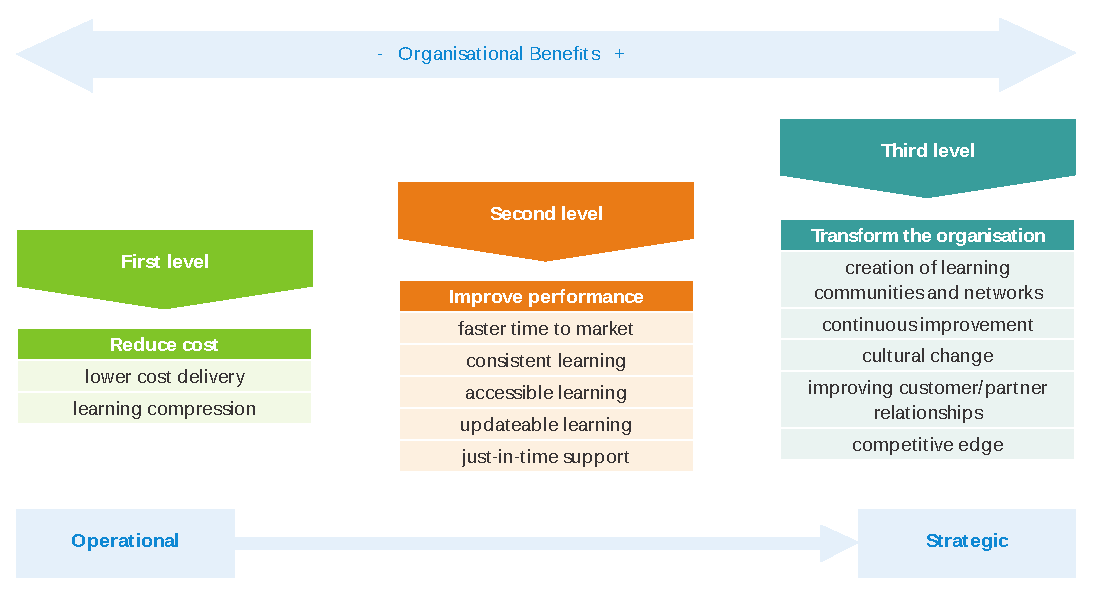
\includegraphics{organisational_benefits}
    \caption[Benefits]{Organisational benefits of e-learning}
    \label{fig:Organisational benefits}
\end{figure}

\subsection{Speed of learning}
In addition to lower delivery costs there is a
strong argument that e-learning is more cost-effective because there is a
reduction in training time known as learning compression. This effect can speed
up the pace at which new employees get the necessary calification. This is
because the single largest cost of training in organisations is the cost of
staff attending the training course, rather than the direct delivery costs in
terms of trainers, course materials, travel and accommodation. E-learning can
deliver benefits by reducing the time it takes to train people because:
\begin{itemize}
\item Learners can go at their own pace, not at the pace of the slowest member of a group, or someone gets left behind
\item Time in classrooms can be spent on questions / topics introduced by other delegates that are irrelevant to the needs of the individual learner
\item There is less time spent on social interaction
\item It takes less time to start and wind up a learning session
\item There is less travel time to and from a training event, or commuting to school
\item Learners learn what they need to learn, they can skip elements of a program they don’t need
\end{itemize}
According to \citet{brandonhall} these factors can add up to an average
compression (saving of learning time) of 35-45 percent when a course is taken
out of the classroom and delivered in an electronic format.

\subsection{Environmental issues}
Taking classes online can help the environment, by reducing waste and C02.  The
Open University study examined in detail energy costs associated with classroom
learning in terms of CO2 emissions, and compared these to the costs of learning
via a computer. Computers are no environmental clean: They burn energy at least
0.125 kwh for a desktop PC, and can contain toxic materials such as lead,
cadmium, and PCB’s that pose serious health and environmental hazards. Despite
this, the CO2 emission levels associated with computer use were significantly
less than those associated with more conventional instructional delivery
methods, and much of the studying was done from home using computers that
students already owned, meaning that it would not change the balance in any way.

By taking lessons online, one can also save trees by saving paper. Many
e-learning courses are entirely self-contained, presenting all learning content
online, or providing alternatives to paper-based forms of communication through
such tools as email, PDF manuals, synchronous classrooms, and other web-based
tools, and there's no need to print out materials at all.

\subsection{Non-discrimitory environment}
The MOOC is open and invitational. No one who wishes to participate is excluded;
people negotiate the extent and nature of their participation according to their
individual needs and wishes, regardless of whether those needs are defined, for
example, by personal interest or workplace requirements. From a theoretical
perspective, this creates a very broad form of “legitimate peripheral
participation”\citep{wegner} which allows individuals to be drawn into the
community of practice at whatever rate is comfortable. From a pragmatic
perspective, this framework pro-vides access to large numbers of people who
might otherwise be excluded for reasons ranging from time, to geographic
location, to formal prerequisites, to financial hardship\citep{wegner}.

\subsection{Time-Proofing}
If a course is well prepared, little to no guidance is necessary from the
teacher, and the knowledge can passed on for extended periods of time. With the
advances in storage technology, online courses can be kept basically forever, at
a low cost of storage, and basically zero cost for duplication.
% 2 pages

\section{The advent of MOOC}
% history, university of reddit, infographics
\subsetion{The first attempts}
Before hitting the online realm, distance learning appeared in the form of
correspondence courses, broadcast courses and early forms of
e-learning\citep{history_of_instr_tech}. Over 4 million Americans
- far more than attended traditional colleges - were enrolled in correspondence
courses by the 1920s, covering hundreds of practical job-oriented topics. Their
completion rate was under 3\%\citep{pursuit_of_knowledge}.

Broadcast radio was new in the 1920s and with programs that were free to
audiences of any size.\citep{listening_in} By 1922, New York University operated its own radio
station, with plans to broadcast practically all its courses. Other schools
followed, including Columbia, Harvard, Kansas State, Ohio State, Purdue,
Wisconsin, Utah and many others. Students read textbooks and listened to
broadcast lectures, while mailing in answers to tests. Journalist Bruce Bliven
asked: "Is radio to become a chief arm of education? Will the classroom be
abolished and the child of the future be stuffed with facts as he sits at home
or even as he walks about the streets with his portable receiving-set in his
pocket?". Completion rates were very low, cheating was hard to detect, and
there was no way to collect tuition. By the 1940s radio courses had virtually
disappeared in the United States.\citep{before_mooc} The Australian School of the Air used
two-way shortwave radio starting in 1951 to teach students in classrooms in
remote locations, with students able to ask questions of the live instructor.

\subsection{The early approaches}
The first MOOCs emerged from the open educational resources (OER) movement. The
term MOOC was coined in 2008 by Dave Cormier of the University of Prince Edward
Island and Senior Research Fellow Bryan Alexander of the National Institute for
Technology in Liberal Education in response to a course called Connectivism and
Connective Knowledge (also known as CCK08). CCK08, which was led by George
Siemens of Athabasca University and Stephen Downes of the National Research
Council, consisted of 25 tuition-paying students in Extended Education at the
University of Manitoba, as well as over 2200 online students from the general
public who paid nothing. All course content was available through RSS feeds
and online students could participate through collaborative tools, including
blog posts, threaded discussions in Moodle and Second Life meetings.\citep{cck08}
Stephen Downes considers these so-called cMOOCs to be more "creative and
dynamic" than the current xMOOCs, which he believes "resemble television shows
or digital textbooks."\citep{courses_lack_of_creativity}

Galway based online education provider ALISON is often cited in industry
literature as the first MOOC, pioneering the systematic aggregation of online
interactive learning resources made available worldwide with a freemium
model. Its stated objective is to enable people to gain basic
education and workplace skills.Contrary to other MOOC providers with
close links to American third level institutions such as MIT and Stanford
University, the majority of ALISON's learners are located in the developing
world with the fastest growing number of users in India. It records 1.2
million unique visitors per month with 250,000 graduates of its 500+ courses as
of January 2013. In February 2014, ALISON registered its 3 millionth user.

%America
\section{MOOC in North America}
Several well-financed American providers emerged, associated with top
universities, including Udacity, Coursera, edX.

In the fall of 2011 Stanford University launched three courses. The first of
those courses was Introduction Into AI, launched by Sebastian Thrun and Peter
Norvig. Enrollment quickly reached 160,000 students. The announcement was
followed within weeks by the launch of two more MOOCs, by Andrew Ng and Jennifer
Widom. Following the publicity and high enrollment numbers of these courses,
Thrun started a company he named Udacity and Daphne Koller and Andrew Ng
launched Coursera. Coursera subsequently announced university partnerships with
University of Pennsylvania, Princeton University, Stanford University and The
University of Michigan.

Concerned about the commercialization of online education, MIT created the
not-for-profit MITx. The inaugural course, 6.002x, launched in March 2012.
Harvard joined the group, renamed edX, that spring, and University of
California, Berkeley joined in the summer. The initiative then added the
University of Texas System, Wellesley College and Georgetown University.

In November 2012, the University of Miami launched its first high school MOOC as
part of Global Academy, its online high school. The course became available for
high school students preparing for the SAT Subject Test in biology.
\citep{history_of_a_revolution}

In January 2013, Udacity launched its first MOOCs-for-credit, in collaboration
with San Jose State University. In May 2013 the company announced the first
entirely MOOC-based Master's Degree, a collaboration between Udacity, AT\&T and
the Georgia Institute of Technology, costing \$7,000, a fraction of its normal
tuition.

In March 2013, Coursolve piloted a crowdsourced business strategy course for 100
organizations with the University of Virginia. A data science MOOC began in
May 2013.

In May 2013 Coursera announced free e-books for some courses in partnership with
Chegg, an online textbook-rental company. Students would use Chegg's e-reader,
which limits copying and printing and could use the book only while enrolled in
the class. In June 2013, the University of North Carolina at Chapel Hill
launched Skynet University, which offers MOOCs on introductory astronomy.
Participants gain access to the university's global network of robotic
telescopes, including those in the Chilean Andes and Australia. It incorporates
YouTube, Facebook and Twitter.

In September 2013, edX announced a partnership with Google to develop Open edX,
an open source platform and its MOOC.org, a site for non-xConsortium groups to
build and host courses. Google will work on the core platform development with
edX partners. In addition, Google and edX will collaborate on research into how
students learn and how technology can transform learning and teaching. MOOC.org
will adopt Google's infrastructure.

EdX currently offers 94 courses from 29 institutions around the world (as of
November 2013). During its first 13 months of operation (ending March 2013),
Coursera offered about 325 courses, with 30\% in the sciences, 28\% in arts and
humanities, 23\% in information technology, 13\% in business and 6\% in
mathematics. Udacity offered 26 courses. Udacity's CS101, with an enrollment
of over 300,000 students, was the largest MOOC to date.

% Europe
\section{MOOC in Europe}
Iversity is a MOOC provider in Germany. With over 82,000 students (Nov 2013)
iversity's "The Future of Storytelling" is Europe's largest MOOC to date.

OpenupEd is a supranational platform, founded with support of the European
Union (EU).

In Ireland ALISON provides free online certificate/diploma courses to two 2
million learners worldwide. ALISON was shortlisted in June 2013 by
London–based education technology company Edxus Group and specialist media and
advisory firm IBIS Capital, as one of the 'top 20 e-learning companies in
Europe' as judged by an expert panel.

In March 2013, a young entrepreneur Volkan Karabacak has started UniversitePlus
online courses system in Turkey to serve the region in Turkish, Russian, Arabic,
and other languages used in EurAsia. It is growing so fast by getting support
from higher education institutions from Turkey, Europe, and United States.

In October 2013, the French government announced the creation of France
Universite Numerique (FUN), a French public alternative to existing solutions.
French business schools have begun launching their own MOOCs, the first being
supervised by Alberto Alemanno.
% 3 pages
\section{Advantages of MOOC}

MOOC's have an economic edge over traditional education: not only it is cheaper
to train students online, but it can provide a stream o revenue for
universities: Coursera for example, is experimenting with a freemium model: the
content is given away for free, sometimes even Freely licensed, but the
certification process involves a fee.

Coursera, Udemy, EdX, Udacity are also considering several other business models:
\begin{itemize}
\item Certification
\item Employers paying to recruit talented students
\item Students résumés and job match services
\item Sponsored high-tech skills courses
\item Enterprises pay to run their own training courses
\item Tuition fees
\end{itemize}

Course developers could charge licensing fees for educational institutions that
use its materials. Introductory or "gateway" courses and some remedial courses
may earn the most fees. Free introductory courses may attract new students to
follow-on fee-charging classes. Blended courses supplement MOOC material with
face-to-face instruction. Providers can charge employers for recruiting its
students. Students may be able to pay to take a proctored exam to earn transfer
credit at a degree-granting university, or for certificates of completion
\citep{profitsofelearning}.

% 2 pages
\section{The problems with MOOC}
Massive open online courses are renowned among academics for their
impressive enrollment figures but also by their unimpressive completion
rates.

% completion rates
Completion rates are typically lower than 10\%, with a steep participation drop
starting in the first week. In the course Bioelectricity, Fall 2012 at Duke
University, 12,725 students enrolled, but only 7,761 ever watched a video, 3,658
attempted a quiz, 345 attempted the final exam, and 313 passed, earning a
certificate.\citep{mooc_completion_rates}

Early data from Coursera suggest a completion rate of 7\%–9\%, probably due to
huge number of stundents that register on the site, as shown in Figure \ref{fig:The growth of Coursera}
 Most registered students intend to explore the topic rather than complete the course,
according to Koller and Ng. The completion rate for students who complete the
first assignment is about 45 percent. Students paying \$50 for a feature designed
to prevent cheating on exams have completion rates of about 70 percent.

\begin{figure}[p]
    \centering
    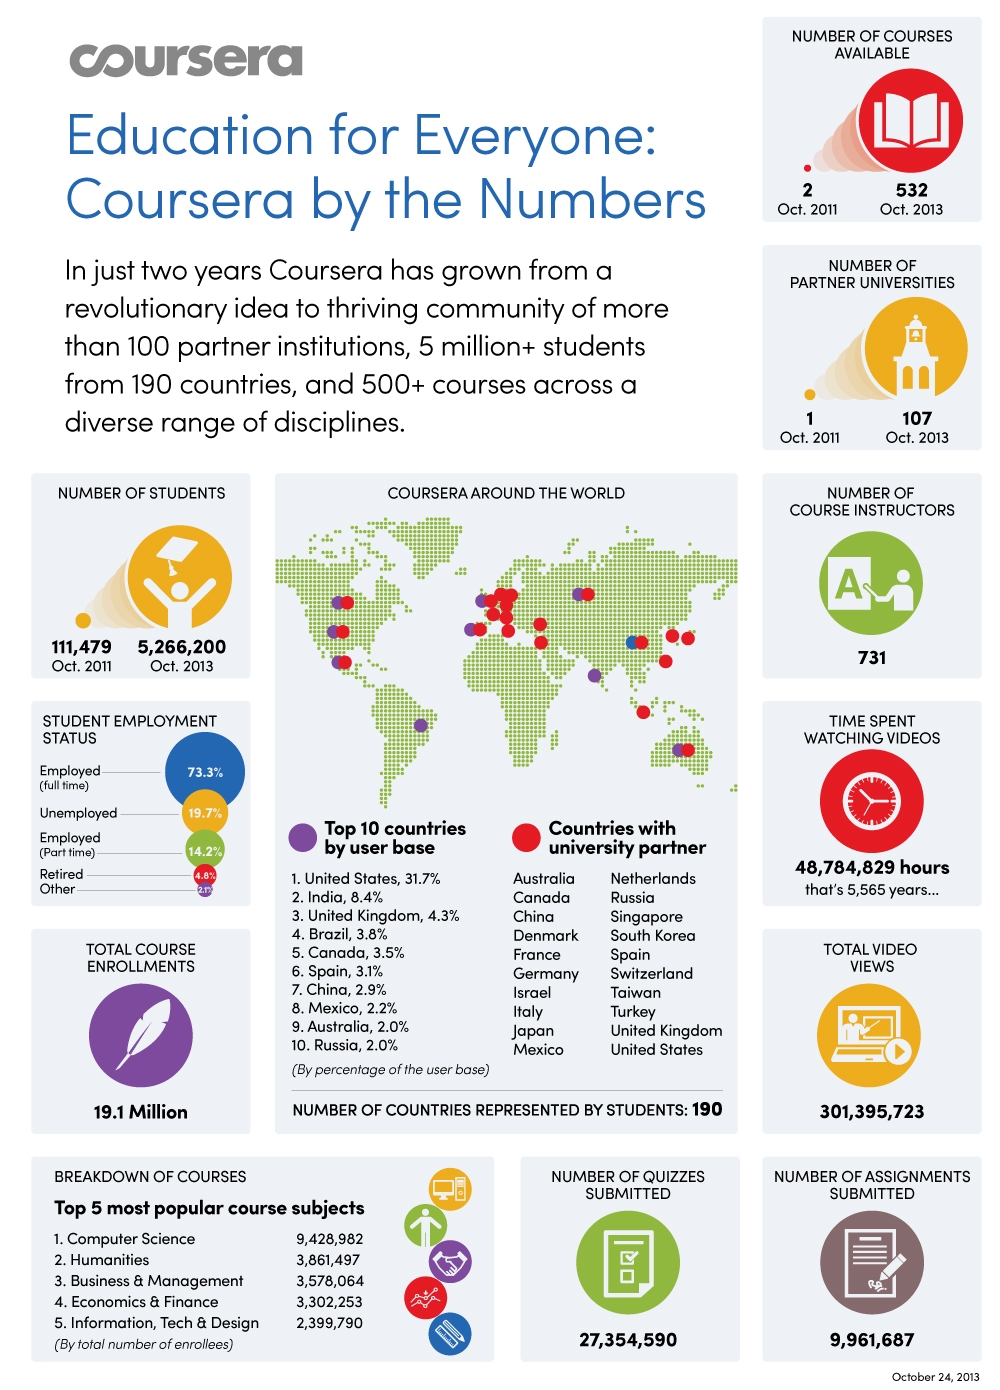
\includegraphics[height=\dimexpr \textheight - 4\baselineskip\relax]{The-Growth-of-Coursera-Infographic}
    \caption[Coursera]{The Growth of Coursera}
    \label{fig:The growth of Coursera}
\end{figure}

One online survey published a "top ten" list of reasons for dropping out.
These were that the course required too much time, or was too difficult or too
basic. Reasons related to poor course design included "lecture fatigue" from
courses that were just lecture videos, lack of a proper introduction to course
technology and format, clunky technology and trolling on discussion boards.
Hidden costs were cited, including required readings from expensive textbooks
written by the instructor that also significantly limited students' access to
learning material. Other non-completers were "just shopping around" when
they registered, or were participating for knowledge rather than a credential.
Providers are exploring multiple techniques to increase the often single-digit
completion rates in many MOOCs.

As a back side to these impressive figures, which often exceed the
total number of students enrolled in large state universities, has been the massive attrition.
Even if millions of students have registered for courses through Coursera, the
company and its university partners have awarded only 280,000 certificates of
completion.

The rates of completion for students who have given some indication that they
plan to do the work is substantially higher. For example, for students who
submit the first assignment, the completion rate jumps to 45 percent.

For students who are paying \$50 for the company’s new Signature Track
program—which includes features designed as safeguards against identity fraud
and cheating on examinations—the pass rates are even higher, at about 70
percent.

That is even higher than the non-Signature Track students who profess
in surveys to high levels of commitment to completing the course. This “suggests
that having skin in the game is highly valuable,” Ms. Koller
said\citep{courseradropout}.
% idea!

Another issue that might arise with MOOC's, is that of identity fraud and cheating
at exams. This might happen in real life too, but facilitated by large crowd of stundent,
and the ease at which one could be relatively anonymous on the internet, these
two issues could reach a large scale, unfortunately.
% 1 page

\section{Towards a better solution}
% tipes of mooc
As MOOCs have evolved, there appear to be two distinct types: those that
emphasize the connectivist philosophy, and those that resemble more traditional
courses. One can distinguish between the two by using the terms "cMOOC" and
"xMOOC", as George Siemens notes it his blog post\citep{moocs_are_a_platform}.
A third type, the "vMOOC", has been suggested to describe
vocational MOOCs, that would require simulations and related technologies to
teach and assess practical skills and abilities.

Such instructional design approaches attempt to connect learners to each other
to answer questions and/or collaborate on joint projects. This may include
emphasizing collaborative development of the MOOC.

One important thing that can help students succeed in an online course is
interpersonal interaction and support says Shanna Smith Jaggars, assistant
director of Columbia University's Community College Research Center. Her
research compared online-only and face-to-face learning in studies of
community-college students and faculty in Virginia and Washington state. Among
her findings: In Virginia, 32\% of students failed or withdrew from for-credit
online courses, compared with 19\% for equivalent in-person courses.\citep{early_report_on_moocs}

Assigning mentors to students is another interaction-enhancing technique.
In 2013 Harvard offered a popular class, The Ancient Greek Hero, taken by
thousands of Harvard students over prior decades. It appealed to alumni to
volunteer as online mentors and discussion group managers. About 10 former
teaching fellows also volunteered. The task of the volunteers, which required
3–5 hours per week, was to focus online class discussion. The instructor,
Gregory Nagy The edX course registered 27,000 students.

% testimonial
As one student, named Rob, was completing a MOOC  from Stanford U Venture Labs, A crash course in
Creativity by Tina Seelig, where about 22,000 were enrolled, reports a rate of
completion of about 50\% completion on their team of 20. The succes is
attributed to using G+ hangouts, that added an engaging social dimension to adult learning.

Unfortunately, MOOCS still have not yet learned to use the tech tools like
real-time chats effectively. With such collaborative tools, a student can learn
more, and create a more engaging environment, that would not be possible otherwise.

So, beside the issue with cheating, the biggest pain point of these systems is that they are
lacking interactivity: most of them are just a site hosting videos, tasks and a forum for students.
These issues can be addressed technically, by inventing something better.

The project that is proposed in this thesis is taking inspiration from several existing projects, that
were mentioned previously.
\begin{itemize}
\item \href{https://coursera.org}{\texttt{Coursera}}
\item \href{https://prezi.com}{\texttt{Prezi}}
\item \href{htpps://iversity.org}{\texttt{Iversity}}
\item \href{https://udacity.com}{\texttt{Udacity}}
\item \href{https://edx.com}{\texttt{Edx}}
\end{itemize}
Prezi is of a special interest, as it has one nice interactive feature: you ca run
a presentation synchronized on several computers. This is a very powerfull feature,
that add one extra dimension to e-learning.
% 2 pages
 % Introduction

% Chapter 2

\chapter{Methods Used}
\label{Chapter2}
\lhead{Chapter 2. \emph{Methods Used}}

\section{Planning}
The application is estimated to reach the beta stage after a month of work, mid
February.
The most complicated part is expected to be the audio/video conference, as this
part of the application represents terra incongnito(a estimated 3 weeks work).
There are very few examples to rely on, and the draft is not yet finalized.
Also, big difficulties lay ahead with the presentation module: is quite hard to
make 20 presentation synchronize with the master one in real-time. It is
expected that this module will take about a week of work.

\section{Test-Driven Development}
Test-Driven Development is a software development methodology and strategy that
requires test to written first (the red stage), then write just enough code to
make the tests pass (the green stage), and the analyze the code written, and
change it if necessary (the refactor stage). By necessity we mean either changing
the code for performance reasons, readability, consistency with the rest of the
code base, or other reasons.

Rspec is the testing framework used for this project.
\subsection{Page-Objects}
Writing plain unit tests, or feature tests comes with one drawback: the tests
can be brittle(if the markup changes), and when a test fails, is usually hard to
tell what caused the fail to happen. Using page objects solves some of this
problem, as when the test fail, the error thrown points to the page that caused
the error.

\section{Software Requirements Specifications}

\subsection{Business requirements}
\begin{enumerate}
\item enables users registration
\item provides a way for users to create courses
\item enable interactive teaching process, featuring video presentation,
doodling
\end{enumerate}

\subsection{User requirements}
\begin{enumerate}
\item registration
\item choosing a course
\item the system should retain the user language preference
\item download materials posted by the teacher
\item chat with the teacher
\item rate the course and teacher
\end{enumerate}

\subsection{Functional requirements}
\begin{enumerate}
\item the application should be internationalised
\item file uploads via AJAX
\item the interface should be responsive (800x600 up to 4k resolution)
\item WebRTC video/audio streams
\end{enumerate}

\subsection{Quality-of-service requirements}
\begin{enumerate}
\item it should work without issues for at least 4 hours
\item each page should have tests
\item each module should be tested with rspec
\item the application should be behavior-driven tested with capybara + RSpec
\item supporting at least up to 200 users simultaneously (apprx. 10-20 courses
at a time)
\item deployment by a skilled administrator should take less than 30 min.
\end{enumerate}

\subsection{Implementation requirements}
\begin{enumerate}
\item the system should not require administrators (self-sustained)
\item there should be no differences between teachers and students outside of a
class
\item avoid loosing data during upgrading and downgrading
\item keep the application independent of the RDBMS solution
\end{enumerate}

\section{Components}
Rails 4 - It finally has support for streaming (with ActionController::Live),
and for server-sent events, that will be used to synchronize the presentation,
doodles.

Another major component will be a browser synchronizer, that will receive
from Rails, via server-sent events, which will dispatch messages to 4 objects
in the course view (Presentation, Media, Sketch and Chat)

\subsection{Storage}
For storing data, the application uses 2 methods: the persistent data is stored
in a SQL database, and the files uploaded by the users are stored in the
file system. For the purpose of archiving the courses there might be implemented
another storage function (for video, chat), but it will not be implemented in
version 1.0 of the application. Chats will be ephemeral, they will only be kept
in users browsers as long as the course is running.

\section{User Interface/User Experience}
Zurb Foundation was chosen as the basis of the application interface. It has
already implemented mos usual widgets, such as buttons, forms, headers, menu.
\subsection{Guidelines}
http://elementaryos.org/docs/human-interface-guidelines

\subsection{Course page}
The most important and complicated page in the whole system is the course page.
It will be a page split in four: the video chat, the text chat, the presentation
and the doodling area.

\section{Implementation}
The project was started by scaffolding a few rails models (course, user), and
integrating components such as Zurb Foundation, creating header/footer, front
page, a course creation form.

\subsection{i18n}
A selector will be provided in the header. On the user profile page this setting
can be chosen permanently. The URL should look like:
discite.info/[lang]/the/rest/of/the/path
 % Methods Used

% Chapter 3

\section{Underlying Technologies}

\subsection{Web as a platform}
One of the major decision when this project was born, was to choose the web as
the underlying platform for the application. The web provides a truly cross-platform
experience, ease of development, good security if best practices are followed.
Discite doesn't use SSL yet, which is a requirement since it do authentication, but
getting a certificate in in the process.

The are other gains by using the web as the basis of the project:
the HTTP protocol, the client-server model and the request-response provides powerful
abstractions and good isolations of components. Isolation means that each time one
makes a change on the server side, is less likely that he will damage the whole platform,
as often happens with other delivery mediums.
The request-response concept, although it provides good isolation of components,
puts the very nature of this application in danger: the goal is to have a highly interactive
application, and that is not possible with such architecture. Fortunately, the very
foundation of the web are being adapted nowadays to the new reality and new requirements.
WebRTC is such a development, one of the most fundamentally changes that web has seen since
it's birth. Another new an powerful feature is Websockets, that are not used
in this project, but were considered along with SSE, Server Sent Events, and the latter was
eventually chosen as the messaging and synchronization technology, due to it's simplicity.

The web as the platform has numerous advatages over the desktop application way
of doing things, including:
\begin{enumerate}[topsep=5pt, partopsep=0pt,itemsep=3pt,parsep=1pt]
\item[--] Good abstractions;
\item[--] Central storage of data;
\item[--] Easy sharing and collaboration;
\item[--] Hardware and OS agnostic.
\end{enumerate}
Another reason to target the web is trying to harness the collective intelligence, one of the most
appealing features that powers the web, and keeps him alive: it's massive amount of users.
% 1 page
\subsection{Ruby on Rails}
% community, activity, embraced TDD
Ruby on Rails is a MVC framework, written in the Ruby language. One of the reasons of the
choice was that it has a big community of developers. The project has been forked 8216 times,
and starred over 22 thousand times at this moment. The \href{https://github.com/rails/rails}{\texttt{rails}}
project at Github has over 2 thousands contributors.
For a developer, this means a large array of choices regarding libraries, a
wealth of tutorials and guides to follow, especially because the community is very
active in this regard: there is lots of training material, paid courses, free courses,
guides on Youtube, and usually great documentation is accompanying each library.
What makes Ruby on Rails stand out of the crowd of development frameworks is
that testing and test-driven development mantra is deeply
integrated in the core of the framework itself, and also in most of the gems
(libraries) that you can use. This makes the environment very stable (as long as you follow
the best practices too), and very easy to develop on.

Understanding the MVC pattern is key to understanding Rails. MVC divides your
application into three layers, each with a specific responsibility.
The Model layer represents your business model (such as Course, User, Person,
Post, etc.) and encapsulates the business logic that is specific to your
application. In Rails, database-backed model classes are derived from
ActiveRecord::Base. Active Record allows you to present the data from database
rows as objects and embellish these data objects with business logic methods.
Although most Rails models are backed by a database, models can also be ordinary
Ruby classes, or Ruby classes that implement a set of interfaces as provided by
the Active Model module.

The Controller layer is responsible for handling incoming HTTP requests and
providing a suitable response. Usually this means returning HTML, but Rails
controllers can also generate XML, JSON, PDFs, mobile-specific views, and more.
Controllers load and manipulate models, and render view templates in order to
generate the appropriate HTTP response. In Rails, incoming requests are routed
by Action Dispatch to an appropriate controller, and controller classes are
derived from ActionController::Base. Action Dispatch and Action Controller are
bundled together in Action Pack.

The View layer is composed of "templates" that are responsible for providing
appropriate representations of your application's resources. Templates can come
in a variety of formats, but most view templates are HTML with embedded Ruby
code (ERB files). Views are typically rendered to generate a controller
response, or to generate the body of an email. In Rails, View generation is
handled by Action View.

Active Record, Action Pack, and Action View can each be used independently
outside Rails. In addition to them, Rails also comes with Action Mailer, a
library to generate and send emails; and Active Support, a
collection of utility classes and standard library extensions that are useful
for Rails, and may also be used independently outside Rails \citep{rails_readme}.
% 3 pages
\subsection{Test-Driven Development}
Test-Driven Development is a software development methodology and strategy that
requires test to written first (the red stage), then write just enough code to
make the tests pass (the green stage), and the analyze the code written, and
change it if necessary (the refactor stage). By necessity we mean either changing
the code for performance reasons, readability, consistency with the rest of the
code base, or other reasons. The upside of this approach is that
the focus is kept on the necessary features. Also, as a refactor is done the
test suite immediately shows if those changes broke any functionality in other
parts of the application.  The downside: the test suite can get as big as actual
code that will be run. But the experience shows that it pays off in the long
term. The gains according to \citep{twelveBenefitsOfUnitTests} are:
\begin{enumerate}[topsep=5pt, partopsep=0pt,itemsep=3pt,parsep=1pt]
    \item[--] Unit tests prove that your code actually works;
    \item[--] You get a low-level regression-test suite;
    \item[--] You can improve the design without breaking it;
    \item[--] It's more fun to code with them than without;
    \item[--] They demonstrate concrete progress;
    \item[--] Unit tests are a form of sample code;
    \item[--] It forces you to plan before you code;
    \item[--] It reduces the cost of bugs;
    \item[--] It's even better than code inspections;
    \item[--] It virtually eliminates coder's block;
    \item[--] Unit tests make better designs;
    \item[--] It's faster than writing code without tests.
\end{enumerate}

There are recent concerns that TDD might induce damage on the architecture of a
application if applied improperly, and mostly due to the complexity of excessive
indirection. Some voices from the community says that coding should be less
about TDD and more about the quality of design decisions.
As usual with such confrontations, consensus is rarely reached, but the thing
that most people agree with is that test-driven development creates a
self-testing code base which is easier to improve later through refactoring, so
TDD gives you a good start point.

\subsubsection{Page Objects}
Writing plain unit tests, or feature tests comes with one drawback: the tests
can be brittle, and if tests fails, is usually hard to
tell what caused the failure. Page objects solves this sort of problem, by
concentrating all the code specific to a page inside the object: data input,
selectors, dropdowns, can be triggered from it. Usually there is a one-to-one mapping
between the pages rendered, and the page objects created. This is not a required though,
but it keeps the number of page objects manageable.
With page objects in place, if a test fails, the error thrown points to the page that caused
the error. A example of such object is presented in Listing~\ref{loginpage}, that encapsulates the
login page.
\begin{lstlisting}[language=Ruby, caption={Login Page object}, label=loginpage]
class LoginPage
  include Capybara::DSL
  include Rails.application.routes.url_helpers

  def initialize(user)
    @user = user
    visit new_user_session_path(:en)
  end

  def login
    fill_in 'email', with: @user.email
    fill_in 'password', with: @user.password
    click_on 'Sign In'
  end
end
\end{lstlisting}

The \textit{LoginPage} class isn't very useful on it's own, but is quite handy when used
in a standard Rspec test, like the one that check if the localization functionality
is working properly, as shown in Listing~\ref{localspec}. If a bug is introduced in the home page (for
example someone deletes the template that renders is), then an error is thrown in
the class \textit{LoginPage}, and this makes debugging easy.

\begin{lstlisting}[language=Ruby, caption={Localization specification}, label=localspec]
require 'spec_helper.rb'
require 'pages/profile_page'
require 'pages/login_page'

describe 'Localized application' do
  let(:user) { build(:user) }
  let(:profile) { ProfilePage.new(user) }

  xit 'should have a language switch' do
    # maybe is necessary to have a global language switch in the navigation bar
  end

  it 'should allow to set default language from profile' do
    profile.locale 'English'
    expect(user.language).to eq('en')
  end

  it 'should use the preffered language on a new session' do
    lang = :ro
    LoginPage.new(user)
    locale_file = File.open(Rails.root + "config/locales/#{lang}.yml")
    title = YAML.load(locale_file)[lang.to_s]['welcome_msg']
    profile.locale 'Romanian'
    visit '/'
    expect(page).to have_content(title)
  end
end
\end{lstlisting}

Tests that begin with \textit{xit} are disabled. In the case of the test presented in
Listing~\ref{localspec}, the code checking whether the language switch from the header is working, due
to the fact that it was never implemented, which was mainly a user experience decision.

\subsection{WebRTC}
Web Real-Time Communication (WebRTC) is a collection of standards, protocols,
and JavaScript APIs, the combination of which enables peer-to-peer audio, video,
and data sharing between browsers (peers). Instead of relying on third-party
plug-ins or proprietary software, WebRTC turns real-time communication into a
standard feature that any web application can leverage via a simple JavaScript
API, provided by the browser.

Delivering rich, high-quality, RTC applications such as audio and video
teleconferencing and peer-to-peer data exchange requires a lot of new
functionality in the browser: audio and video processing capabilities, new
application APIs, and support for half a dozen new network protocols.
Thankfully, the browser abstracts most of this complexity behind three primary
APIs:
\begin{enumerate}
    \item[--]MediaStream: acquisition of audio and video streams;
    \item[--]RTCPeerConnection: communication of audio and video data;
    \item[--]RTCDataChannel: communication of arbitrary application data.
\end{enumerate}
All it takes is a few lines of JavaScript code, and any web application can
enable a rich teleconferencing experience with peer-to-peer data transfers.
That’s the promise and the power of WebRTC. However, the listed APIs are also
just the tip of the iceberg: signaling, peer discovery, connection negotiation,
security, and entire layers of new protocols are just a few components required
to bring it all together.
Signaling is of special importance, most of the clients nowadays are behind routers, firewalls
and Network Address Translation devices, and this would make impossible direct connections with them.
Signaling is the process of coordinating communication.
In order for a WebRTC application to set up a connection, its clients need to exchange information and metadata:
\begin{enumerate}
    \item[--] Session control messages used to open, close and initialize communication;
    \item[--] Error messages;
    \item[--] Media metadata such as codecs and codec settings, bandwidth and media types;
    \item[--] Key data, used to establish secure connections;
    \item[--] Network data, such as a host's IP address and port as seen by the outside world.
\end{enumerate}

This signaling process needs a way for clients to exchange messages.
That mechanism is not implemented by the WebRTC APIs: you need to build it
yourself, or use a third-party service. The reason why a signaling
server must be used, is to avoid clients being trapped outside of the reach.
Signaling was implemented as shown in Listing~\ref{webrtc_con}. In
this case a third-party server is used, provided by nodejitsu, to simplify
deployment and management of the Discite platform.
\begin{lstlisting}[language=JavaScript, caption={WebRTC connection setup}, label=webrtc_con]
// removed code
var SIGNALING_SERVER = 'http://webrtc-signaling.nodejitsu.com:80/',
    defaultChannel = location.hash.substr(1) || location.href.replace(/\/|:|#|%|\.|\[|\]/g, '');

var channel = config.channel || defaultChannel;
var sender = Math.round(Math.random() * 999999999) + 999999999;

io.connect(SIGNALING_SERVER).emit('new-channel', {
    channel: channel,
    sender: sender
});

var socket = io.connect(SIGNALING_SERVER + channel);
socket.channel = channel;
socket.on('connect', function () {
    if (config.callback) config.callback(socket);
});

socket.send = function (message) {
    socket.emit('message', {
        sender: sender,
        data: message
    });
};
// removed code
\end{lstlisting}

The signaling protocol is actually left out of of the WebRTC specification, in order
to allow for different signaling protocol to be implemented (such as SIP, Jingle),
and the way it is used in Discite is the one specified in the JavaScript Session Establishment Protocol
(JSEP), as presented in Figure~\ref{fig:jsep}.
\begin{figure}[ht!]
    \centering
    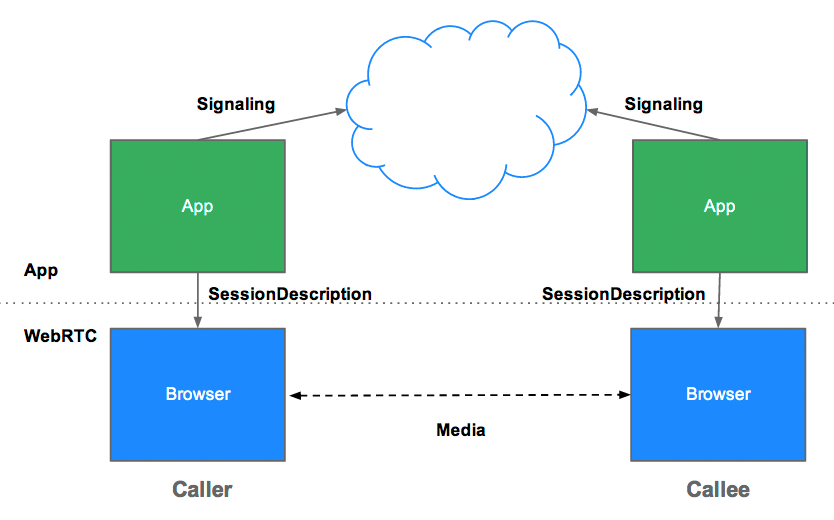
\includegraphics[height=8.5cm]{jsep}
    \caption{JSE protocol architecture}
    \label{fig:jsep}
\end{figure}
After establishing the connection, the application has to ask for streaming from specific
devices. This poses privacy and security issues, and all browsers currently require for
users to approve each time connections to the devices they want to share.
In order to get their permission, the \textit{getUserMedia} API is used, as presented in Listing~\ref{getusermedia}.
\begin{lstlisting}[language=JavaScript, caption={getUserMedia request}, label=getusermedia]
// code removed
      var video = document.createElement('video');
      video.setAttribute('autoplay', true);
      video.setAttribute('controls', true);
      videosContainer.insertBefore(video, videosContainer.firstChild);
      getUserMedia({
          video: video,
          onsuccess: function (stream) {
              config.attachStream = stream;
              video.setAttribute('muted', true);
              callback();
      }
  });
\end{lstlisting}
The application asks for both video and audio streams and by default the streaming starts muted.

Not surprisingly, the architecture and the protocols powering WebRTC also
determine its performance characteristics: connection setup latency, protocol
overhead, and delivery semantics, to name a few. In fact, unlike all other
browser communication, WebRTC transports its data over UDP. However, UDP is also
just a starting point. It takes a lot more than raw UDP to make real-time
communication in the browser a reality \citep{high_perf_browser}.

\subsection{deck.js}
\textit{deck.js} is A JavaScript library for building modern HTML presentations.
It has replaced a failed attempt to integrate \textit{ViewerJS} into the site, to make possible
to upload .pdf and .odp files, as the library doesn't support yet such a use case\citep{githubissue}.
This strategy will be evaluated in the future, but for the time being, there are several possible solutions:
\begin{enumerate}
    \item[--] upload HTML presentation directly;
    \item[--] allow uploads for .pdf's and .odp, then convert them on the server to HTML, with delayed-job and a separate worker;
    \item[--] upload .pdf's and .odp, integrate \textit{ViewerJS} in the front-end;
    \item[--] custom HTML slides editor.
\end{enumerate}
At the moment the first solution is in use, the third option has failed thus
far, there were attempts to do the second, but it complicates deployment.
The last one seems like a good option, but there wasn't enough time to explore it.

On the other hand, \textit{deck.js} is flexible enough to let advanced CSS and JavaScript authors make
highly customized decks, but also provides templates and themes for the HTML novice to build a standard
slideshow. The themes are actually not provided yet(one cannot choose what theme
his deck should use), just one of them is compressed and minified inside the assets pipeline.
\textit{deck.js} was integrated via Bower, and the necessary HTML attached to the
course rendered in a view template, as shown in Listing~\ref{deckjstemp}.
\begin{lstlisting}[language=Python, caption={deck.js template}, label=deckjstemp]
%h4 #{@course.title}, by #{@course.user.handle}, lasts #{@course.duration} hours
#presentation
  %div{"aria-role" => "navigation"}
    %a.deck-prev-link{href: "#", title: "Previous"}
    %a.deck-next-link{href: "#", title: "Next"}
  %form.goto-form{action: ".", method: "get"}
    %label{for: "goto-slide"} Go to slide:
    %input#goto-slide{list: "goto-datalist", name: "slidenum", type: "text"}/
    %datalist#goto-datalist
    %input{type: "submit", value: "Go"}/
  = render file: @slides_path
\end{lstlisting}
The \textit{deck.core} module provides all the basic functionality for creating and
moving through a deck. It applies and removes classes to indicate the state of
the deck and its slides, allowing CSS to take care of the visual representation
of each state. It also provides methods for interacting with the deck, as well
as basic key bindings for going to the next and previous slides. On top of these
basic feature, more advanced one are build, such as jumping to a specific slide, showing
the number of slide and so on. Separate extension modules provide more
functionality using the API provided by core \citep{imakewebthings}.

There are still conflicts between the CSS provided by \textit{deck.js}, the CSS from \textit{Zurb Foundation},
but most of them were solved by adding more CSS. In the pursuit to tackle this problem,
one idea that was tried was to use an iframe, that would basically make a new window
inside the browser, with it's own stylesheets and Javascript, but this wasn't feasible,
as another server was needed to stream the HTML in the iframe. This would make the application
considerably harder to maintain and deploy, so the idea was dropped.
% half a page
% move this part of the table of contents in a new page
\addtocontents{toc}{\protect\newpage}
%
\subsection{Technologies and frameworks}
In the process of building the application, a big part of the weight lifting was done by third
party libraries and frameworks. Otherwise the project would be impossible to implement by
one person. Many libraries were installed, tested, integrated, and some thrown away for
various reason.
A brief list of technologies used:
\begin{enumerate}[topsep=5pt, partopsep=0pt,itemsep=3pt,parsep=1pt]
    \item[--] Ruby - A dynamic, free programming language with a focus on
        simplicity and productivity.
        It has an elegant syntax that is natural to read and easy to write.
        \href{https://wwww.ruby-lang.org/en/}{\texttt{www.ruby-lang.org/en}};
    \item[--] \href{http://rubyonrails.org}{\texttt{Ruby on Rails}} - a MVC
        (Model-View-Controller) server-side web development framework, backed by
        the Ruby language;
    \item[--] \href{http://foundation.zurb.com/}{\texttt{Zurb Foundation}} - A
        responsive front-end framework;
    \item[--] \href{https://github.com/plataformatec/devise}{\texttt{Devise}} for
        authentication;
    \item[--] \href{http://www.webrtc.org/}{\texttt{WebRTC}} Real-Time Communication
        implemented in browser, with a simple JavaScript API.
\end{enumerate}

Ideally, the system should not require administrators and be as self-sustained as possible.
This is achievable with cloud computing, continous integration, and other such techniques.
Using Rails migration features, we try to avoid loosing data during upgrading/downgrading and
by taking advantage by another abstraction provided by Rails, namely ActiveRecord, the application
is kept independent of the RDBMS solution.

Ruby on Rails recently acquired support for streaming (with ActionController::Live),
and for server-sent events, that will be used to synchronize the presentations.
The project was started by scaffolding a few rails models (course, user), and
integrating components such as Zurb Foundation, creating header/footer, front
page, a course creation form.

These technologies were chosen because of previous experience with them, and because they
are well tested and widely deployed on production environments.
The only new and untried technology is WebRTC: is a very young project, aiming
to enable creation of rich web applications with HTML5. It's still a
\href{http://dev.w3.org/2011/webrtc/editor/webrtc.html}{\texttt{draft}} at W3C.
Nonetheless, the technology is already implemented in 2 popular browser: Google
Chrome and Mozilla Firefox.  Internet Explorer doesn't yet support it, but as
it's market share is below 10\%, we can assume that more than 80\% of web users
\citep{browserStats} will be able to use the program. As the specification will
leave the draft stage, even more supported browsers are expected.

\subsubsection{Storage systems used}
For storing data, the application uses 2 methods: the persistent data is stored
in a SQL database, and the files uploaded by the users are stored in the
file system. For the purpose of archiving the courses there might be implemented
another storage function (for video, chat), but it will not be implemented in
version 1.0 of the application. Chats will be ephemeral, they will only be kept
in users browsers as long as the course is running.

\subsection{Software Requirements Specifications}
In order for the platform to be of useful an provide value to it's end-users, a set of business
requirements have to be met such as:
\begin{enumerate}[topsep=5pt, partopsep=0pt,itemsep=3pt,parsep=1pt]
    \item[--] enables users registration;
    \item[--] provides a way for users to create courses;
    \item[--] enable interactive teaching process, featuring video presentation, doodling.
\end{enumerate}

For users to be able to use the system safely and effectively, the system must be carefully designed
so students will find the platform familiar. To achieve that, several user requirements have
to be met:
\begin{enumerate}[topsep=5pt, partopsep=0pt,itemsep=3pt,parsep=1pt]
    \item[--] registration;
    \item[--] choosing a course;
    \item[--] the system should retain the user language preference;
    \item[--] download materials posted by the teacher;
    \item[--] chat with the teacher;
    \item[--] rate the course and teacher.
\end{enumerate}

Another spot were he application has received attention, is in the functional requirements department:
the application is intended to reach on as many platforms as possible (computers, tablets, phones), and and
as many users as possible. Phones with a certain screen resolution are not supported, unfortunately, as it
would cripple the whole experience for other users, but recent smartphones
should do the job. This means that the application should:
\begin{enumerate}[topsep=5pt, partopsep=0pt,itemsep=3pt,parsep=1pt]
    \item[--] have localizaton and internationalisation;
    \item[--] support file uploads via AJAX;
    \item[--] the interface should be responsive (800x600 up to 4k resolution);
    \item[--] WebRTC video/audio streams.
\end{enumerate}

To avoid frustration while using the site, some performance and quality-of-service requirements
must reached:
\begin{enumerate}[topsep=5pt, partopsep=0pt,itemsep=3pt,parsep=1pt]
    \item[--] it should work without issues for at least 4 hours;
    \item[--] each page should have tests;
    \item[--] each module should be tested with rspec;
    \item[--] the application should be behavior-driven tested with capybara + RSpec;
    \item[--] supporting at least up to 200 users simultaneously (apprx. 10-20 courses at a time);
    \item[--] deployment by a skilled administrator should take less than 30 min.
\end{enumerate}

 % User testing

% Chapter 4

\section{Architecture}
\label{sec:Architecture}
% UML diagrams, source code, SSE, ERD diagrams
The software was built following the Ruby on Rails conventions, namely the MVC (Model-View-Controller)
pattern. A more accurate name would be Model-Controller-View, if is to show the
depth in the software stack of each component. The Model is the one interacting with the
database (managed by MySQL, or in our case PostgreSQL). The controllers are sending and
receiving data, filtering it, send redirect headers, and rendering templates. The Views
are the components that the user gets to see them, they are templates that are rendered
on the browsers, and interpolate data made available by the controller.
The \textit{Course} model shown in Listing~\ref{course} is the most important in the system.
It doesn't do much, it defines a relation to the \textit{User} model and has some validations
that prevent users from abusing the system.
\begin{lstlisting}[language=Ruby, caption={Course Model}, label=course]
# @author Dumitru Ursu
# Model for courses
class Course < ActiveRecord::Base
  belongs_to :user
  has_attached_file :slides
  validates_attachment_content_type :slides, content_type: [
    'application/vnd.oasis.opendocument.presentation', 'application/pdf',
    'text/html']
end
\end{lstlisting}
Switching from Rails 3.1 to the 4-th version, made the model even more compact, by implementing
\textit{ActiveModel::Model}. The new version also allows create a new class and be able to update its attributes through a form,
like an \textit{ActiveModel} object, but not persist it to the database.
Previously the attributes were listed within the model,but now they are only present in the
\textit{CourseController} filters and migrations. In the class diagram of the system the attributes
and methods are also shown, in Figure~\ref{fig:Class Diagram}.
\begin{figure}[ht!]
    \centering
    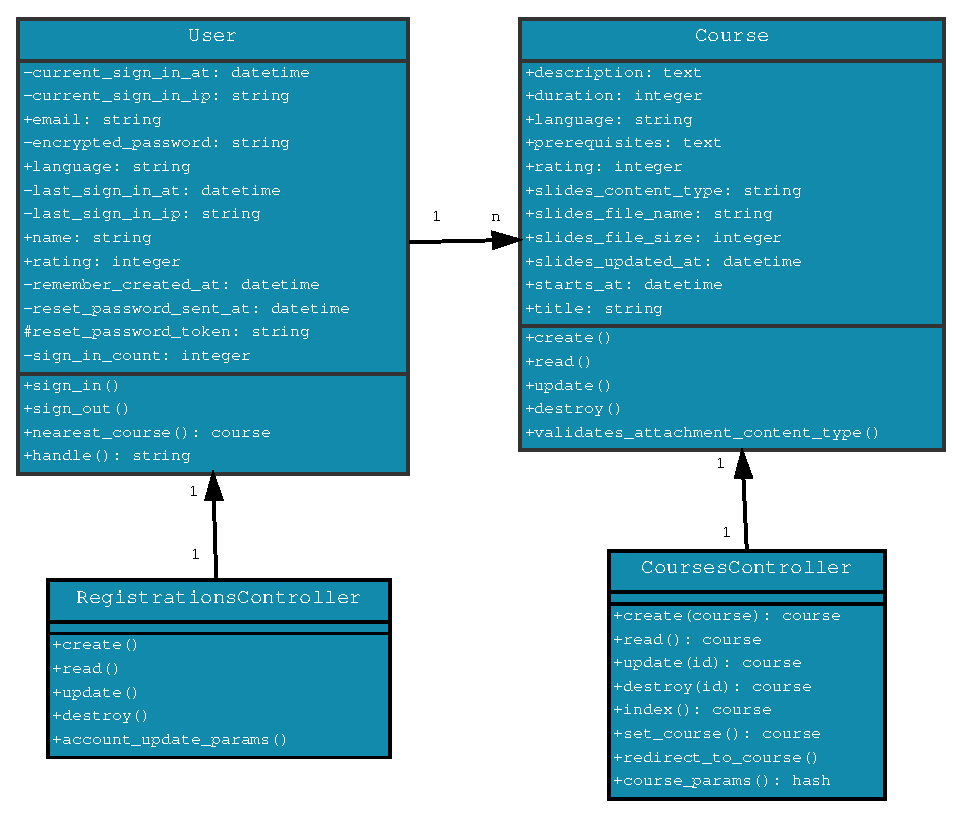
\includegraphics{class}
    \caption{Class diagram of system components}
    \label{fig:Class Diagram}
\end{figure}

\subsection{Rails migrations}
Rails provides a mechanism to modify the database schema, and also keeping all the
data in place, if one is careful enough. Migrations use a Ruby DSL so that one
doesn't have to write SQL by hand, allowing the schema and changes to be database
independent. For example, in Listing~\ref{slidesmig} several columns are added
with the \textit{add\_attachment} command. It may not be seem so, but this DSL predicate
is provided by \textit{PaperClip}, a library that ease easy file attachment library for
Active Record.
\textit{PaperClip} \textit{add\_attachment} wraps 4 attributes:
\begin{enumerate}
    \item[--] $\langle attachment\rangle$\_file\_name;
    \item[--] $\langle attachment\rangle$\_file\_size;
    \item[--] $\langle attachment\rangle$\_content\_type;
    \item[--] $\langle attachment\rangle$\_updated\_at.
\end{enumerate}
The \textit{Paperclip} attributes are all prefixed with that attachment's name, in this case
the HTML file that is being uploaded as a presentation.
This allows to have multiple attachments per model, and give them a friendly front end.
The intent behind it was to keep setup as easy as possible and to treat files as much like other attributes as possible.
The next features that will be implemented with \textit{PaperClip} is avatars for users.
\begin{lstlisting}[language=Ruby, caption={Slides migration}, label=slidesmig]
class AddSlidesColumnToCourses < ActiveRecord::Migration
  def self.up
    add_attachment :courses, :slides
  end

  def self.down
    remove_attachment :courses, :slides
  end
end
\end{lstlisting}
The \textit{self.down} event is triggered when the database is reverted to a previous state,
past the point when this migration was created. All migrations are timestamped
to keep track of how the database was created, and in what order should the database
be rolled back  as shown in this listing \ref{ls_migrations}. \begin{lstlisting}[language=Bash, caption={The migration directory}, label=ls_migrations]
20130923040646_devise_create_users.rb
20131005225555_create_courses.rb
20131031112018_add_rating_to_courses.rb
20131031112055_add_rating_to_users.rb
20140210142725_add_name_to_users.rb
20140210174537_add_duration_to_courses.rb
20140213021746_add_language_to_users.rb
20140228161213_add_slides_column_to_courses.rb
\end{lstlisting}
These are not created by hand, (although one could create the files like that),
instead most of the time Rails developers rely on a migrations generator. The
names of the migrations are self-explanatory.

\subsection{Client-side architecture}
As mentioned at the beginning of the Chapter~\ref{sec:Architecture}, the interface is generated from the views file.
The views in their turn interact with the controller. It is possible to access the models
directly form the views, but this is bad practice, as the user interfaces gets mixed with
business logic, and becomes very hard to change. This requests paths and interaction between
the mentioned Rails components is shown in Figure~\ref{rails_mvc}.
\begin{figure}[ht!]
\centering
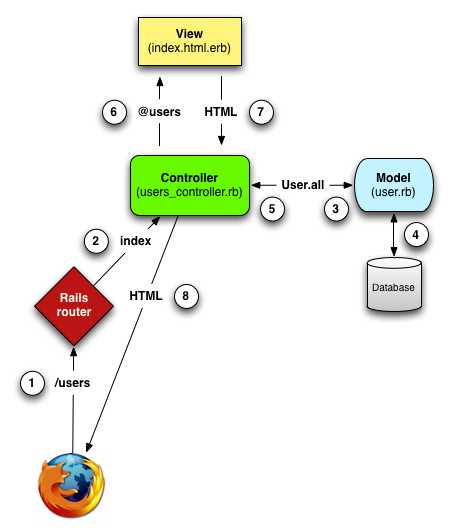
\includegraphics[height=10cm]{rails_mvc}
\caption{Rails components interaction}
\label{rails_mvc}
\end{figure}

The views use a special templating language: by default is .erb, which stands for
embedded ruby, and is basically HTML with a new tag for embedding ruby scripts,
but in Discite it was replaced with Haml (HTML abstraction markup language). Haml
looks and feels a lot like Python code, in the sense that is very concise and it
relies on indentation for scoping, instead of braces or tags. This can be seen in
Listing~\ref{courseform}, where the form for creating, editing and updating courses
is described. This might seem like a long and intricate form, but it is
rendered in over 250 lines of pure HTML, and is rendered in the browser window as shown
in Figure~\ref{fig:course_creation}.
\begin{lstlisting}[language=Python, caption={Course creation template}, label=courseform]
= form_for @course, :html => { :multipart => true } do |f|
  - if @course.errors.any?
    #error_explanation
      %h2= "#{pluralize(@course.errors.count, "error")} prohibited this course from being saved:"
      %ul
        - @course.errors.full_messages.each do |msg|
          %li= msg
  .row
    .columns.large-8.small-6
      = f.label :title
      = f.text_field :title
    .columns.large-4.small-6
      = f.label :language
      = f.select :language, LanguageList::COMMON_LANGUAGES.map{ |language| [language.name, language.iso_639_1] }
  = f.label :description
  = f.text_area :description, rows: 8
  = f.label :prerequisites
  = f.text_area :prerequisites, rows: 6
  = f.label 'Slides'
  = f.file_field :slides
  .row
    .columns.large-10
      = f.label 'Starting Date'
      = datetime_select :course, :starts_at, {time_separator: '', datetime_separator: '',
        prompt: true}, {class: 'large-2 columns end'}
    .columns.large-2
      = f.label 'Duration (hours)'
      = f.text_field :duration, type: 'number'
  = f.submit 'Save', class: 'button'
\end{lstlisting}

\subsection{Assets management}
A subsystem of Rails takes care of minifying and compressing CSS and JavaScript
files. This system is called the asset pipeline.
Beside the aforementioned features, the pipleline also has the ability to write
these assets in other languages and pre-processors such as CoffeeScript, Sass
and ERB and the templating language of choice from this project, Haml.
The asset pipeline is no longer a core feature of Rails 4, it has been extracted
out of the framework into the \textit{sprockets-rails} gem, and in fact, most of it's job
is done by Bower in this project.
Bower is a package manager for the web, built by Twitter. It offers a generic
solution to the problem of front-end package management, while exposing the
package dependency model via an API that can be consumed by a more opinionated
build stack, in this case the Rails default asset pipeline. There are no system
wide dependencies, no dependencies are shared between different apps, and the
dependency tree is flat.

Like some other similar projects, Bower runs over Git, and is package-agnostic.
It was the only one that was reliable enough, and provide enough packages for this
project, after several failed attempts. A packaged component can be made up of any type of asset, and
use any type of transport. In this project case, we use git and SSH protocol to get
the data in the project, then commit it, and then is pushed to the server via SSH.
One way of optimizing this process would be to concatenate the server on the local
machine, and then send them to the remote server, but this has yet to be investigated.

As more CSS frameworks, the JavaScript librariels began to clump up
the project, it became clear that the standard pipeline could no longer handle the management of the assets.
At this time, in fact sprockets still concatenates, minifies and compresses assets, but the way they are
installed in the project is different, as seen in Figure \ref{fig:deployment}
\begin{figure}[ht!]
    \centering
    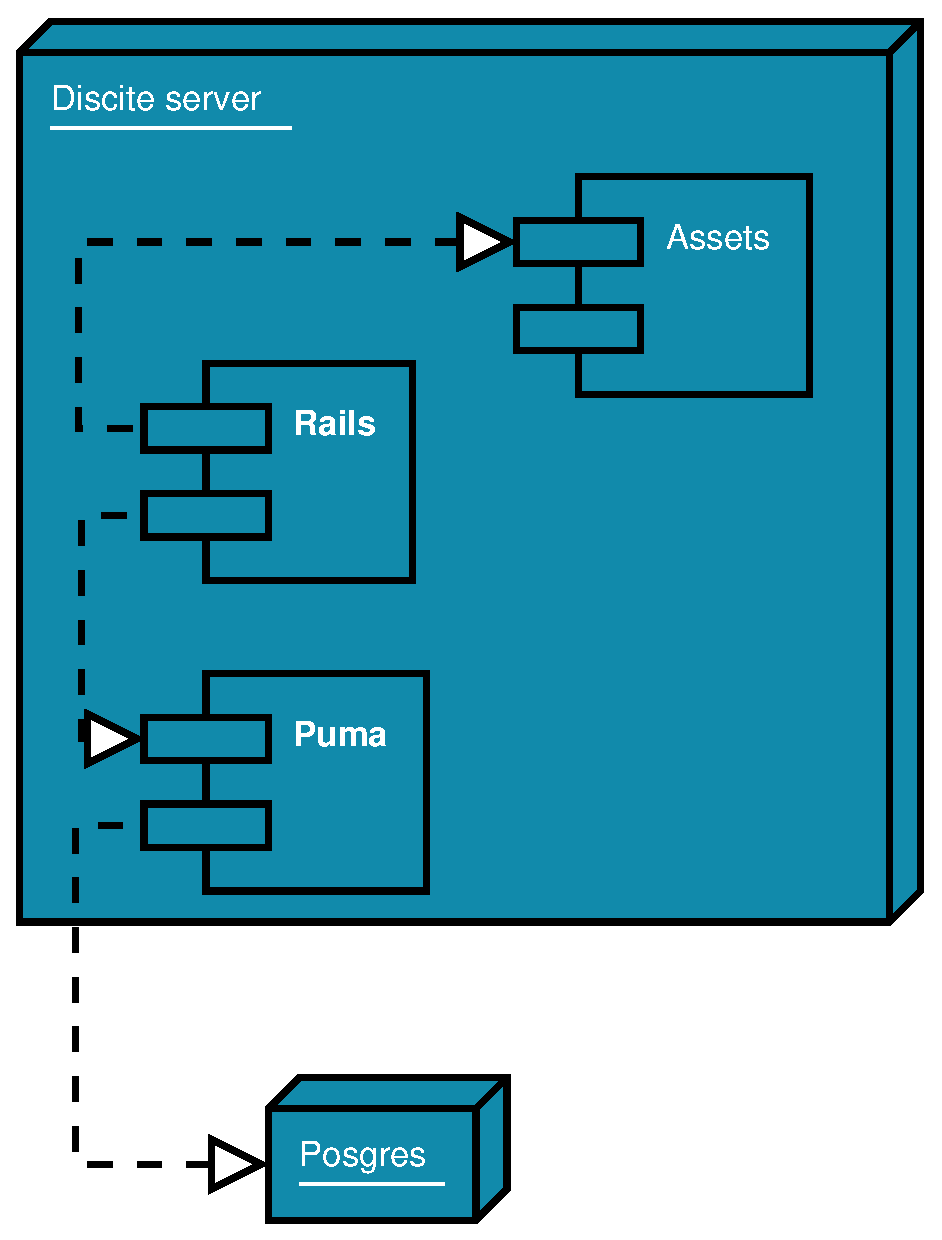
\includegraphics[height=8cm,keepaspectratio]{deployment}
    \caption{Deployment diagram}
    \label{fig:deployment}
\end{figure}

Some of the trials and errors with asset management ranged from purely using the
pipepline (which has been inadequate for this project), to using git submodules,
manually installing JS files, jammit, and systems that gemify automatically
libraries from git repositories.
In this case, accommodating Rails and Bower was quite a easy and scalable way to go.
\begin{lstlisting}[language=JavaScript, caption={Bower.json file}, label=bower]
version": "0.0.1",
  "authors": [
    "Dumitru Ursu <dima@ceata.org>"
  ],
  "description": "\"A peer to peer teaching network\"",
  "main": "bower.json",
  "moduleType": [
    "globals"
  ],
  "license": "MIT",
  "homepage": "discite.info",
  "private": true,
  "ignore": [
    "**/.*",
    "node_modules",
    "bower_components",
    "vendor/assets/components",
    "test",
    "tests"
  ],
  "dependencies": {
    "deck.js": "~1.1.0",
    "deck.annotate.js": "~0.0.0",
    "sisyphus": "1.1.103",
    "foundation": "5.2.2",
    "jquery": "2.1.0",
  }
}
\end{lstlisting}

Assets installed this way need to be loaded into sprokets, so minification, concatenation and compression
will happen automatically, and this is done in Listing~\ref{enable_bower}.
\begin{lstlisting}[language=Ruby, caption={Plugging Bower into the assets pipeline}, label=enable_bower]
module Discite
  class Application < Rails::Application
    # Application configuration should go into files in config/initializers
    # -- all .rb files in that directory are automatically loaded.
    config.i18n.enforce_available_locales = true
    config.i18n.load_path += Dir[Rails.root.join('config', 'locales', '*.{rb,yml}').to_s]
    config.i18n.default_locale = :en
    config.assets.paths << Rails.root.join('app', 'assets', 'fonts', 'vendor', 'components')
  end
end
\end{lstlisting}

\subsection{Storage}
There are 2 main type of storage used by the Discite platform: \textit{localStorage} and  \textit{PosgreSQL}
The first is used by a library called \textit{Sysiphus}, that saves HTML forms data to
\textit{localStorage} to restore them after browser crashes, tabs closings and other
disasters. This way, our users will not have to refill the form for course creation,
if anything bad happens and as the form has become quite big, this was a very welcomed improvement.
The course creation process is shown in Figure~\ref{fig:course_management}.
\begin{figure}[ht!]
    \centering
    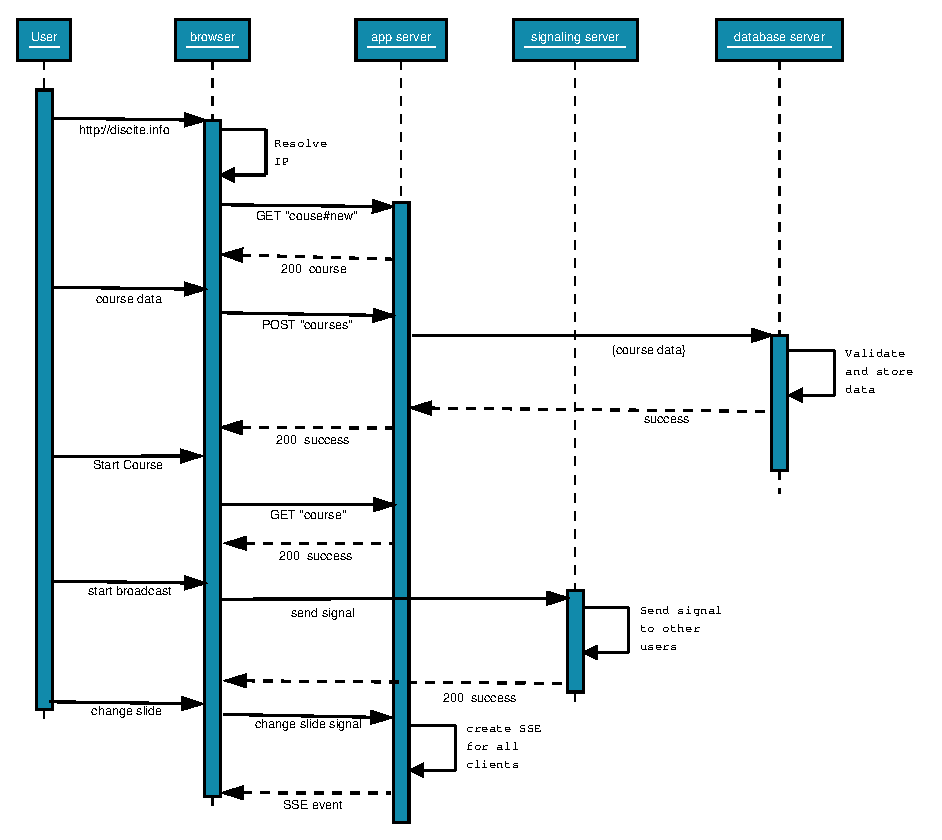
\includegraphics[height=20cm,width=\textwidth, keepaspectratio]{s_course_management}
    \caption{Sequence diagram for course management}
    \label{fig:course_management}
\end{figure}

\textit{localStorage} is a  way for web pages to store named key/value pairs locally, within
the client web browser. Like cookies, this data persists even after you navigate
away from the web site, close your browser tab, exit your browser. Unlike
cookies, this data is never transmitted to the remote web server
(unless you specifically do that). Unlike all previous
attempts at providing persistent local storage, it is implemented natively in
web browsers, so it is available even when third-party browser plugins are not.

The second type of storage is on the server side, where PostgreSQL is used,
often simply "Postgres",that is an object-relational database management
system (ORDBMS) with an emphasis on extensibility and standards-compliance. As a
database server, its primary function is to store data, securely and supporting
best practices, and retrieve it later, as requested by other software
applications, be it those on the same computer or those running on another
computer across a network (including the Internet). It can handle workloads
ranging from small single-machine applications to large Internet-facing
applications with many concurrent users. Recent versions also provide
replication of the database itself for security and scalability.

In fact, ActiveRecord provides some nice abstractions around the whole SQL concept,
and Posgres can be easily exchanged for another RDBMS vendor that has support
with ActiveRecord, such as MySQl, Oracle, or MSSQL.
ActiveRecord allows programmers to programmatically define a schema in a
portable DSL. This means you can define tables, indexes, etc. without using SQL
directly, so your applications can more easily support multiple databases, as shown in Listing~\ref{arschema}.
\begin{lstlisting}[language=Ruby, caption={ActiveRecord Schema definition}, label=arschema]
ActiveRecord::Schema.define do
  create_table :users do |t|
    t.string :name, null: false
  end

  add_index :users, :name

  create_table :posts do |t|
    t.integer :user_id, null: false
    t.string :name
    t.text :body
    t.boolean :private, default: false
  end

  add_index :posts, :author_id
end
\end{lstlisting}

This comes at a price though, as more advanced features that PostgreSQL supports are
being left out of the abstraction, like HStore.
HStore functions much like serializing hashes, except that data can be queried
much faster since HStore is a native data type. It is not  supported natively in
Rails 4, but until then we’ll need to use the \textit{activerecord-postgres-hstore} gem,
and this would make our code depend on a specific RDBMS. When this is not an
issue, higher performance can be gained from this move, as \textit{Course}
and \textit{User} models can be stored directly as hashes, without going though
several cycles of serialization/deserialization.
This functionality requires a recent version of PostgreSQL that supports the HStore
extension.The extension can be enabled by running the migration from Listing~\ref{hstore_enable}.
\begin{lstlisting}[language=Ruby, caption={Enable HStore Postgres extension}, label=hstore_enable]
class SetupHstore < ActiveRecord::Migration
  def self.up
    execute "CREATE EXTENSION hstore"
  end

  def self.down
    execute "DROP EXTENSION hstore"
  end
end
\end{lstlisting}

After this is done, it is possible to create a column with a type of HStore, here
we are giving our User model a column called data with HStore type.

\begin{lstlisting}[language=Ruby, caption={Hstore for User model}, label=hstore_course]
class CreateUser < ActiveRecord::Migration
  def change
    create_table :user do |t|
      t.string  :name
      t.hstore  :data
      t.timestamps
    end
  end
end
\end{lstlisting}
Users can then be created by following the user registration process, presented in the Figure~\ref{fig:user_creation},
or by creating them manually, at Rails console, like in Listing~\ref{hstore_user_creation}.
The second process could be of use if a university or school is doing mass-enrollment of students,
and already has their data, or the registration page is taken down, to stop unknown people from registering
on the website, basically making it a private site.
\begin{figure}[ht!]
    \centering
    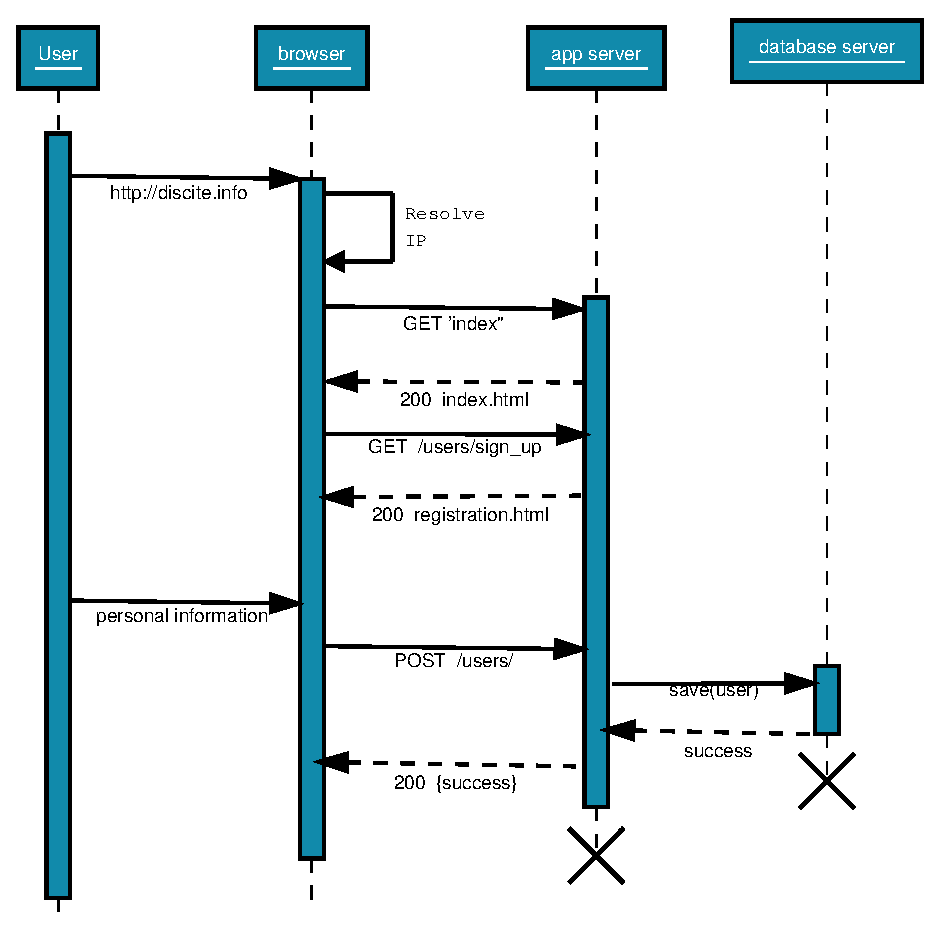
\includegraphics[height=13cm]{s_user_creation}
    \caption{Sequence diagram for user creation}
    \label{fig:user_creation}
\end{figure}

\begin{lstlisting}[language=Ruby, caption={Creating a new User}, label=hstore_user_creation]
User.create(:name => "George Popescu", :data => {'email' => 'g.popescu@gmail.com', 'age' => 18, 'group' => '11B'})
User.last.data['age']  # => 18
\end{lstlisting}


This kind of persistent storage is used for user data and courses. The hierarchical filesystem is used to
store the presentation files. Storing them in the RDBMS is considered, but was not
implemented because there were no reasons for it yet, but scalability and integrity of
data might become a concern for the slides files.
Moving files in the RDMS brings some advantages, like the following:
\begin{enumerate}
    \item[--] When storing files in the database there is a guarantee that the data
        is consistent. The foreign keys will enforce referential integrity. It
        is relatively hard to execute transactional operations on both the file
        system and the database at the same time. This is the most important
        reason why the switch should be made;
    \item[--] When all the user generated data is in the database it is easier
        to maintain. In order to backup the data we will only backup the database.
        While it is not that hard to backup some files it is still a
        concern and is spreading the effort and the area where errors can occur.
        What is more, if at some point there is a change in
        the application that requires some update to the existing data like
        changing the file names to match some convention or adding a watermark
        to the slides it is easier to manipulate data using SQL than writing a
        custom tool to crawl through files and directories, and having more services
        to maintain;
    \item[--] One can store file related metadata like file size, image
        dimensions, filenames  and make queries over it:  if this data is
        "attached" to the file and it is easier to preserve data integrity.
\end{enumerate}

\subsection{Future Architetural Improvements}
One major improvement would be implementation of a management dashboard for the teacher, to allow better course
management. The software is does not currently provide means to block abusive students, for example. A set of
features that are planned at latter versions are:
\begin{enumerate}
    \item[--] System for sorting, and approving students;
    \item[--] A enrollment key system;
    \item[--] PDF support for presentations;
    \item[--] Ratings for students and courses;
    \item[--] Featured courses/teachers;
    \item[--] HTML editor for presentations, based on Scribe from Guardian.
\end{enumerate}

The search system that is based on \textit{FortyFacets}, a library for
building explorative search interfaces, implemented as shown in Listing~\ref{search} is
not working reliably, and doesn't support users/teacher searches for the moment.
\begin{lstlisting}[language=Ruby, caption={Course Search controller}, label=search]
class CourseSearch < FortyFacets::FacetSearch
    model 'Course'
    text :title
    range :duration, name: 'Duration'
    facet :language, name: 'Language'
    facet :starts_at, name: 'Starting date', order: :starts_at
    facet :rating, name: 'Rating', order: :rating
  end
\end{lstlisting}

The User search shown in Listing~\ref{user_search} poses privacy concerns, and can't have a full implementation at the moment.
Most of the fieds are stripped away (email, age) due to these concerns. The best solution found
is to have Privacy Preferences inside the profile page, but this requires a highly elaborate User model,
and lots of tweaking to the system, so it won't crash if the needed data is not made availble.
\begin{lstlisting}[language=Ruby, caption={User search controller}, label=user_search]

  class UserSearch < FortyFacets::FacetSearch
    model 'User'
    text :name
    #add rating to to user search
  end

  def courses
    @search = CourseSearch.new(params) # this initializes your search object from the request params
    @course = @search.result.paginate(page: params[:page], per_page: 5) # optionally paginate through your results
  end

  def users
    @search = UserSearch.new(params)
    @user = @search.result.paginamte(page: params[:page], per_page: 5)
  end
end
\end{lstlisting}

The biggest leap forward will be achieved if the course page will be rewritten:
a better choice for doing the signaling would have been WebSockets, and
Nodejs with socket.io as is shown in benchmarks to support la larger number of users
that ActiveController::Live is capable of for the moment.
The current implementation is quite simple, as shown in listing \ref{syncronizer}

\begin{lstlisting}[language=Ruby, caption={ActionController::Live syncronizer}, label=syncronizer]
require 'streamer/sse'

class SlidesController < ApplicationController
  include ActionController::Live

  def index
      # SSE expects the `text/event-stream` content type
    response.headers['Content-Type'] = 'text/event-stream'

    sse = Streamer::SSE.new(response.stream)

    begin
      sse.write(params.permit(:slide), event: 'slide_change')
    rescue IOError
      # When the client disconnects, we'll get an IOError on write
    ensure
      sse.close
    end
    render nothing: true
  end
end
\end{lstlisting}

\subsubsection{Service Oriented Architecture}
Because of the possible rewrite of the application core feature, the course page,
an alternative architecture is considered. The current monolithic architecture is
hard to change, and hard to adapt to changes. On the bright side, the application is easy
to deploy, having only one component to take care of, and this is done so by design.

A service-oriented architecture is essentially a collection of services. These
services communicate with each other via a certain protocol. The communication can involve either
simple data passing or it could involve two or more services coordinating some
activity. Some means of connecting services to each other is needed, and for this
a REST API might be considered, which is a popular way to consume and create services,
as it's easy to create, read, update or delete information on a server using simple HTTP calls.

\clearpage

 % Conclusions


%% ----------------------------------------------------------------
% Now begin the Appendices, including them as separate files

\addtocontents{toc}{\vspace{2em}} % Add a gap in the Contents, for aesthetics

\appendix % Cue to tell LaTeX that the following 'chapters' are Appendices

% Appendix A

\chapter{Maintenace Manual}
\label{AppendixA}
\lhead{Appendix A. \emph{Maintenance Manual}}

% how an administrator should proceed in order to deploy the application
% and to maintain it fuctional
 % User's Manual

% Appendix B

\chapter{Maintenace Manual}
\label{AppendixB}
\lhead{Appendix B. \emph{Maintenance Manual}}

Write your Appendix content here.
 % Maintenance Manual

% Appendix C

\chapter{Design Documents}
\label{AppendixC}
\lhead{Appendix C. \emph{Design Documents}}

Write your Appendix content here.
 % Design Documents

% Appendix D

\chapter{Source Code}
\label{AppendixD}
\lhead{Appendix D. \emph{Source Code}}

Write your Appendix content here.
 % Source Code

% Appendix E

\chapter{Test Suite}
\label{AppendixD}
\lhead{Appendix D. \emph{Test Suite}}

% let's define some commands to include the test suite
\newcommand{\lTest[1]}{\lstinputlisting[style=ruby]{/home/dimon/sandbox/rails/discite/spec/\string#1}}
\newcommand{\lFeatureTests[1]}{\lstinputlisting[style=ruby]{/home/dimon/sandbox/rails/discite/spec/features/\string#1}}
\newcommand{\lPagesTests[1]}{\lstinputlisting[style=ruby]{/home/dimon/sandbox/rails/discite/spec/pages/\string#1}}


\lTest[spec_helper.rb]

\lFeatureTests[home_spec.rb]

\lPagesTests[home_page.rb]
 % Test Suite

\addtocontents{toc}{\vspace{2em}}  % Add a gap in the Contents, for aesthetics
\backmatter

%% ----------------------------------------------------------------
\label{Bibliography}
% Change the left side page header to "Bibliography"
\lhead{\emph{Bibliography}}
% Use the "unsrtnat" BibTeX style for formatting the Bibliography
\bibliographystyle{unsrtnat}
% The references (bibliography) information are stored in the file named
% "Bibliography.bib"
\bibliography{Bibliography}

\end{document}  % The End
%% ----------------------------------------------------------------
